\section{Pengendalian Aliran}

Sebuah layanan dalam satu sistem sering kali bertugas untuk mengerjakan sesuatu dan memanggil layanan lain. Dalam kasus ini, terdapat kemungkinan munculnya masalah kinerja dan keandalan ketika layanan mengalami beban yang tinggi. Keadaan ini dapat menciptakan situasi \textit{backpressure}.

Dalam konteks perangkat lunak, \textit{backpressure} dapat didefinisikan sebagai \textit{resistance or force opposing the desired flow of data through software} \parencite{backpressureExplained}. Selain melakukan penyesuaian pada sumber daya sistem, terdapat tiga strategi yang dapat digunakan untuk menangani \textit{backpressure}, yaitu:

\begin{enumerate}
    \item Mengurangi kecepatan produsen mengirimkan pesan.
    \item Menggunakan \textit{buffer} untuk sementara mengakumulasikan pesan.
    \item Membuang (\textit{drop}) sebagian pesan yang diterima.
\end{enumerate}

Pola penyeimbangan beban berbasiskan antrean (\textit{Queue-based load leveling}) merupakan pola desain yang menyelesaikan masalah \textit{backpressure} dengan menggunakan antrean yang bertindak sebagai \textit{buffer} antara pesan dengan sebuah layanan, sehingga beban dapat dikontrol dan layanan tetap berjalan dengan stabil \parencite{queueLoadLeveling}.

\begin{figure}[htbp]
    \centering
    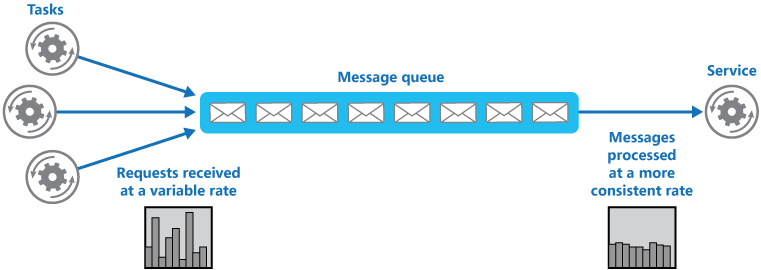
\includegraphics[width=0.8\textwidth]{resources/chapter-2/queue-based-load-leveling-pattern.png}
    \caption{Contoh Pola Penyeimbangan Beban Berbasiskan Antrean \parencite{queueLoadLeveling}}
    \label{fig:queue-based-load-leveling-pattern}
\end{figure}

Penggunaan antrean memisahkan pesan dengan pekerja, sehingga pekerja dapat menangani pesan berdasarkan kemampuannya, terlepas dari banyaknya pekerjaan yang bertambah seiring dengan berjalannya waktu. Pola ini memiliki berbagai keuntungan, seperti menjaga ketersediaan, memaksimalkan skalabilitas, dan membatasi biaya atau penggunaan sumber daya. Meskipun begitu, penggunaan pola ini akan meningkatkan latensi, terlebih lagi apabila pesan yang dikirimkan jauh lebih besar daripada kapasitas pemrosesan pada sistem.